\section{Simulação e choques}
\label{SecChoques}

Compreendidas as relações entre as variáveis através da solução analítica, resta simular o modelo. Nas subseções seguintes, são verificados os efeitos dos seguintes choques:
(i) aumento na taxa de crescimento do investimento residencial; (ii) redução na participação dos salários na renda e;  (iii) aumento na taxa de juros. Antes de prosseguir, a figura \ref{dag} ilustra a hierarquia de determinação em que as setas vão das variáveis mais exógenas em direção às mais endógenas. Em outras palavras, quanto mais ligações determinada variável recebe, mais endógena será e se não receber nenhuma ligação significa que esta variável é determinada exogenamente (como é o caso de $r_m$, $\sigma_{mo}$ $\phi_0$, $\pi$ e $\omega$).
A partir desta ilustração, observa-se a ausência de relação entre crescimento e distribuição, bem como a forma com que os preços dos imóveis afetam o sistema por meio da taxa própria de juros e, consequentemente, a taxa de crescimento dos gastos autônomos e da economia como um todo. 
Dito isso, as simulações (resumidas na tabela \ref{Resumo_Simulacao}) serão comparadas com um cenário \textit{baseline}
correspondente aos primeiros 50 períodos da simulação --- e representado por uma linha tracejada em alguns dos gráficos\footnote{
	Optou-se não apresentar a linha tracejada referente ao \textit{baseline} em alguns dos gráficos facilitar a visualização dos choques.}
 --- enquanto os resultados dos choques estão reunidos na tabela \ref{ResumoChoques}.

\begin{figure}[H]
	\centering
	\caption{Diagrama representativo do modelo}
		\label{dag}
	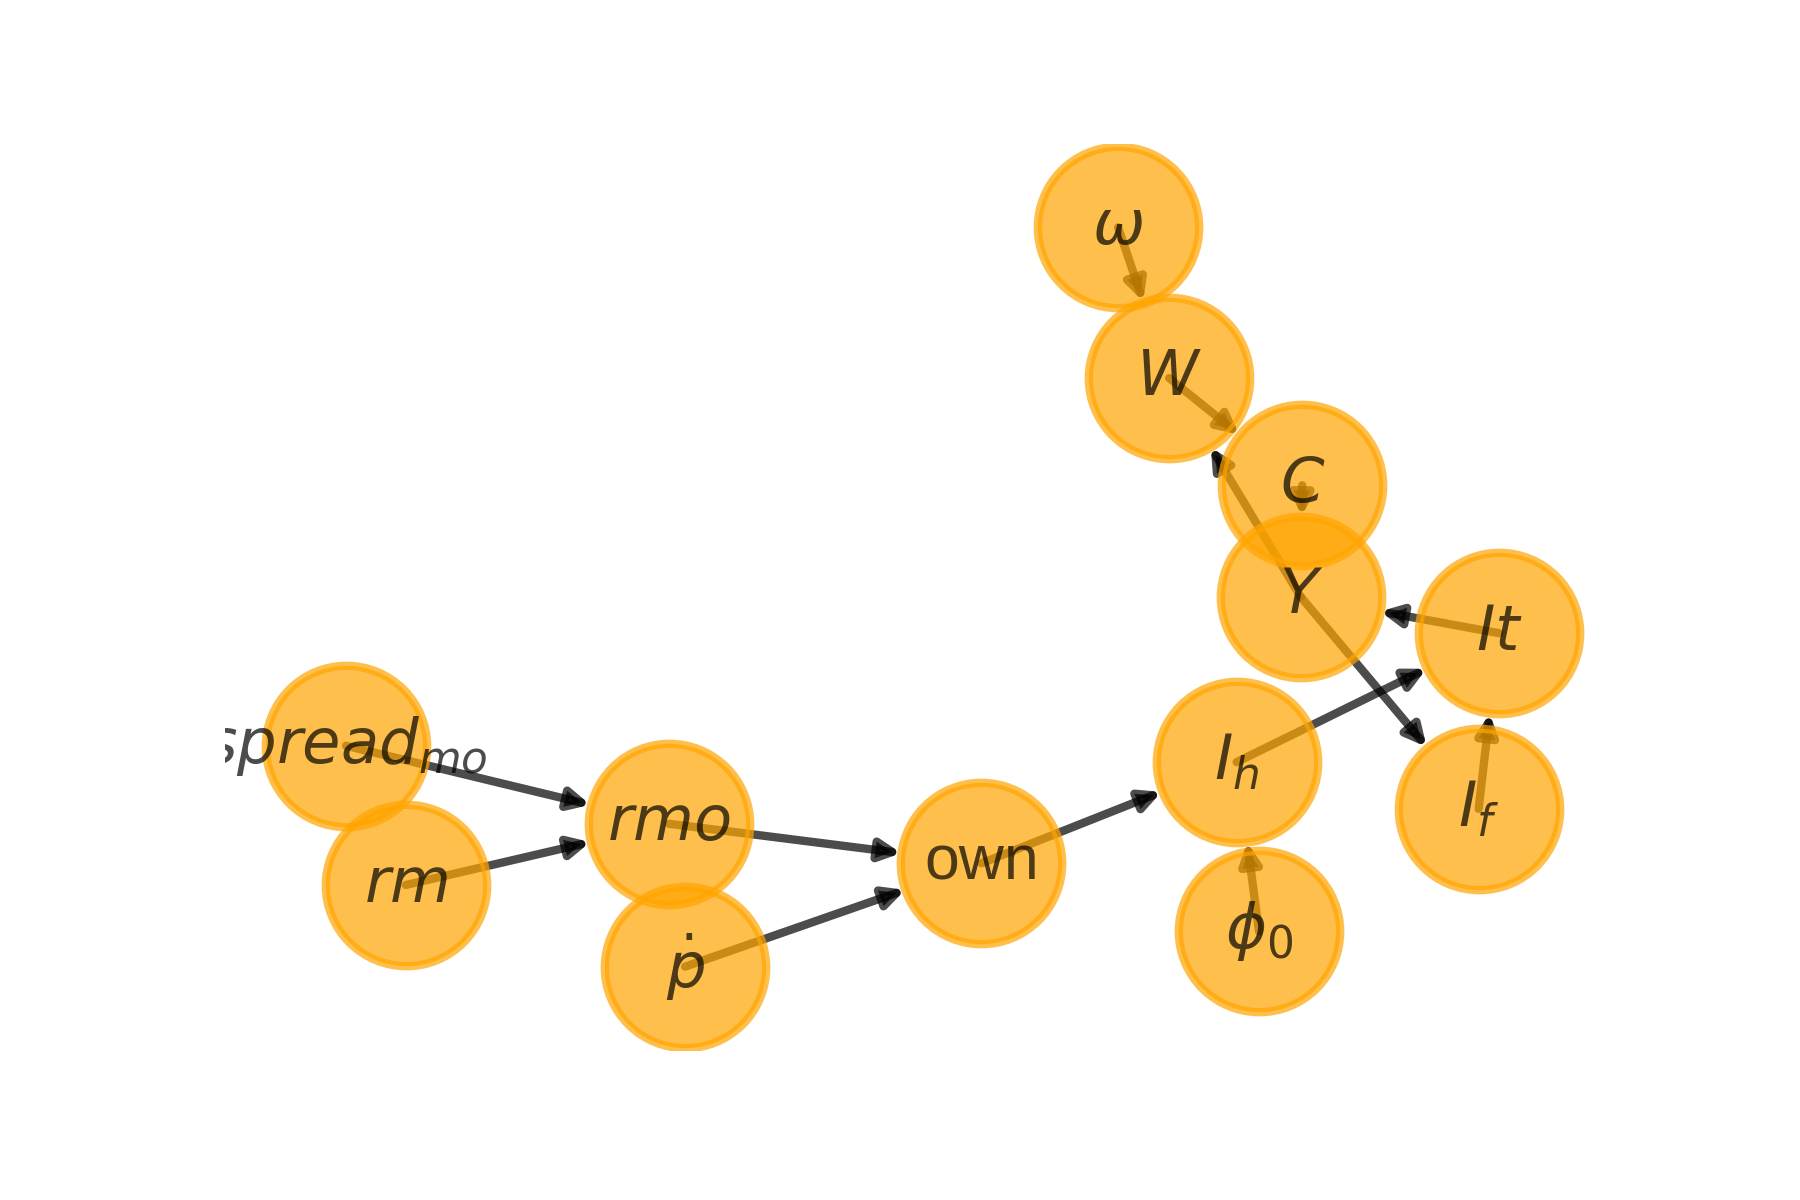
\includegraphics[width=\textwidth]{../../Modelo/Versoes/Dag.png}
	\caption*{\textbf{Fonte:} Elaboração própria}
\end{figure}



\subsection*{Aumento na taxa de crescimento do investimento residencial}

%Um aumento da taxa de crescimento dos gastos autônomos ($\uparrow g_Z$) causa uma maior taxa de crescimento da demanda que, por sua vez, implica em um maior grau de utilização. Em seguida, de acordo com o princípio do ajuste do estoque de capital, as firmas revisam seus planos de investimento e, consequentemente, altera a propensão marginal a investir de forma que o grau de utilização se ajusta lenta e gradualmente ao desejado. No longo prazo, (i) taxa de crescimento da economia converge a taxa dos gastos autônomos; (ii) como resultado, a propensão marginal a investir é permanentemente mais elevada em relação ao \textit{baseline}; (iii) grau de utilização converge ao normal.

Um aumento da taxa de crescimento dos gastos autônomos (seja por um aumento em $\phi_0$ ou na inflação de imóveis) significa uma maior taxa de crescimento da demanda que inicialmente implica um maior grau de utilização da capacidade produtiva. Em seguida, de acordo com o princípio do ajuste do estoque de capital, as firmas revisam seus planos de investimento e, consequentemente, alteram a propensão marginal a investir de forma que o grau de utilização se ajuste lenta e gradualmente ao desejado. A mudança da propensão marginal a investir faz com que  a economia cresça temporariamente mais rápido que os gastos autônomos. Ao fim dos processos de ajustamento: (i) a taxa de crescimento da economia converge a taxa de crescimento dos gastos autônomos; (ii) a propensão marginal a investir é permanentemente mais elevada em relação ao \textit{baseline}; (iii) grau de utilização converge ao normal.


Além disso, como a renda disponível das famílias (capitalistas) passa a crescer a esta taxa mais elevada, o comprometimento da renda disponível com o pagamento de juros se reduz. 
Em outras palavras, o paradoxo da dívida está presente 
uma vez que a taxa de crescimento do estoque de dívida das famílias não supera a da renda apesar do aumento da taxa de crescimento dos gastos financiados por crédito. O mesmo se aplica para o caso das firmas em que a taxa de lucro líquida se aproxima da taxa de lucro bruta ao longo da transição em que a massa de lucro também aumenta. 
Destaca-se também a menor participação do imóveis no estoque de capital total --- tal como indicado pelas equações \ref{partial_phi0} e \ref{partial_pi} --- resultante deste aumento da taxa de crescimento economia inicialmente maior que a taxa de crescimento dos gastos autônomos acompanhado do \textit{overshooting} da taxa de crescimento do investimento das firmas --- isto é, um efeito nível no estoque de capital produtivo --- na tentativa de ajustar o grau de utilização ao normal (figuras \ref{choque_1} e \ref{choque_4}).


\begin{figure}[H]
	\centering
	\caption{Efeito de um aumento no componente autônomo}
	\label{choque_1}
	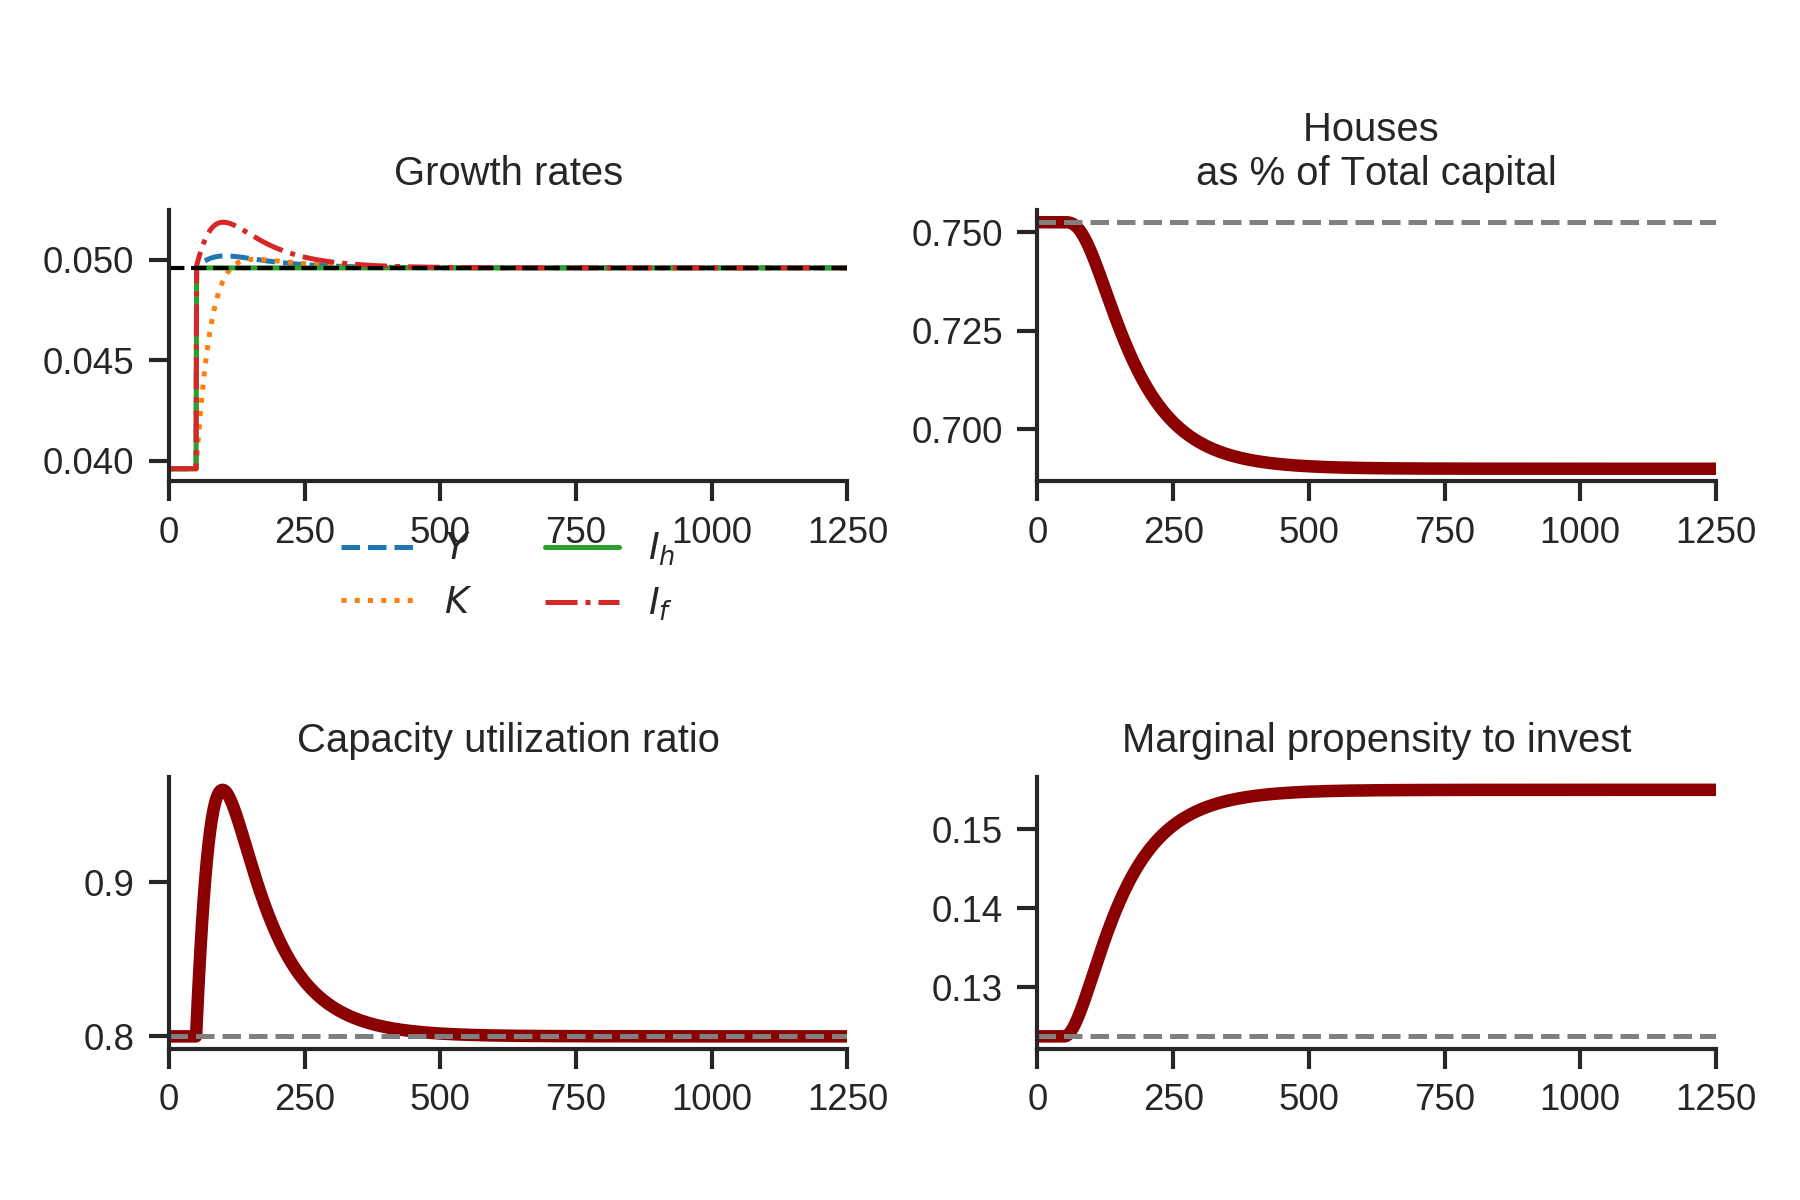
\includegraphics[width=\textwidth]{../../Modelo/Versoes/Shock_1.png}
	\caption*{\textbf{Fonte:} Elaboração própria}
\end{figure}


\begin{figure}[H]
	\centering
	\caption{Efeito de um aumento da inflação de imóveis}
	\label{choque_4}
	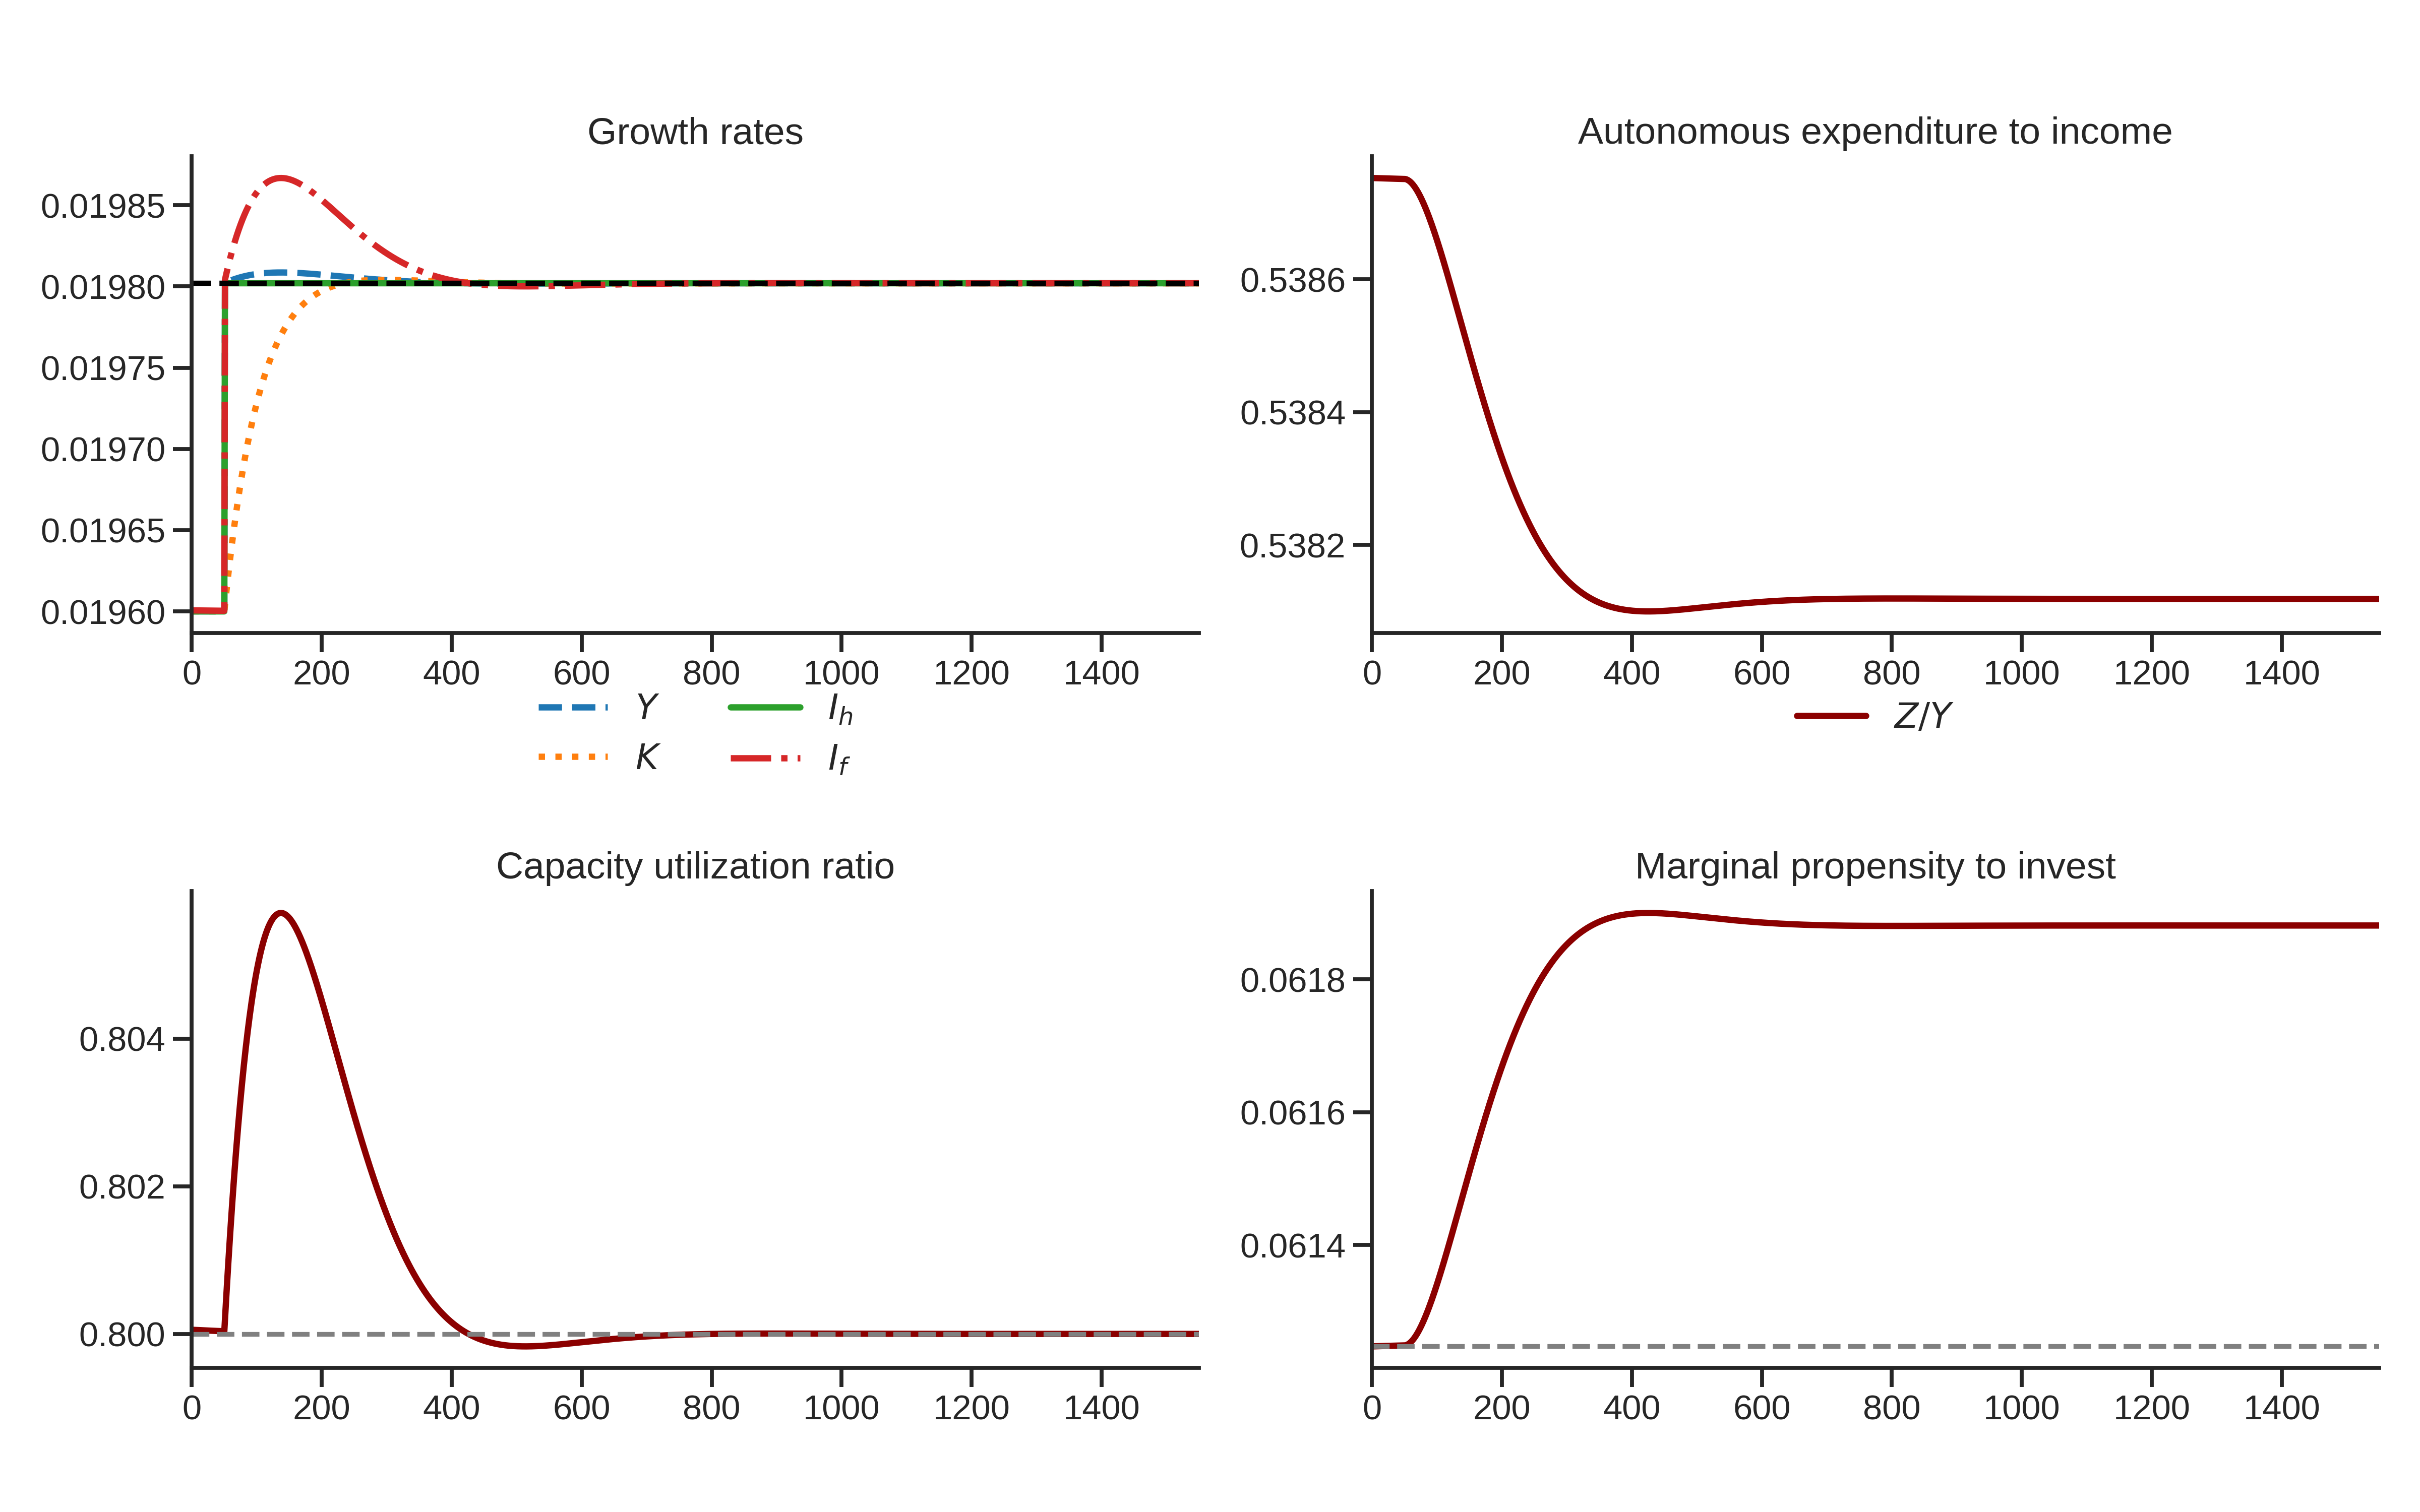
\includegraphics[width=\textwidth]{../../Modelo/Versoes/Shock_4.png}
	\caption*{\textbf{Fonte:} Elaboração própria}
\end{figure}

\begin{figure}[H]
	\centering
	\caption{Efeito de um aumento no componente autônomo}
	\label{choque_1Norms}
	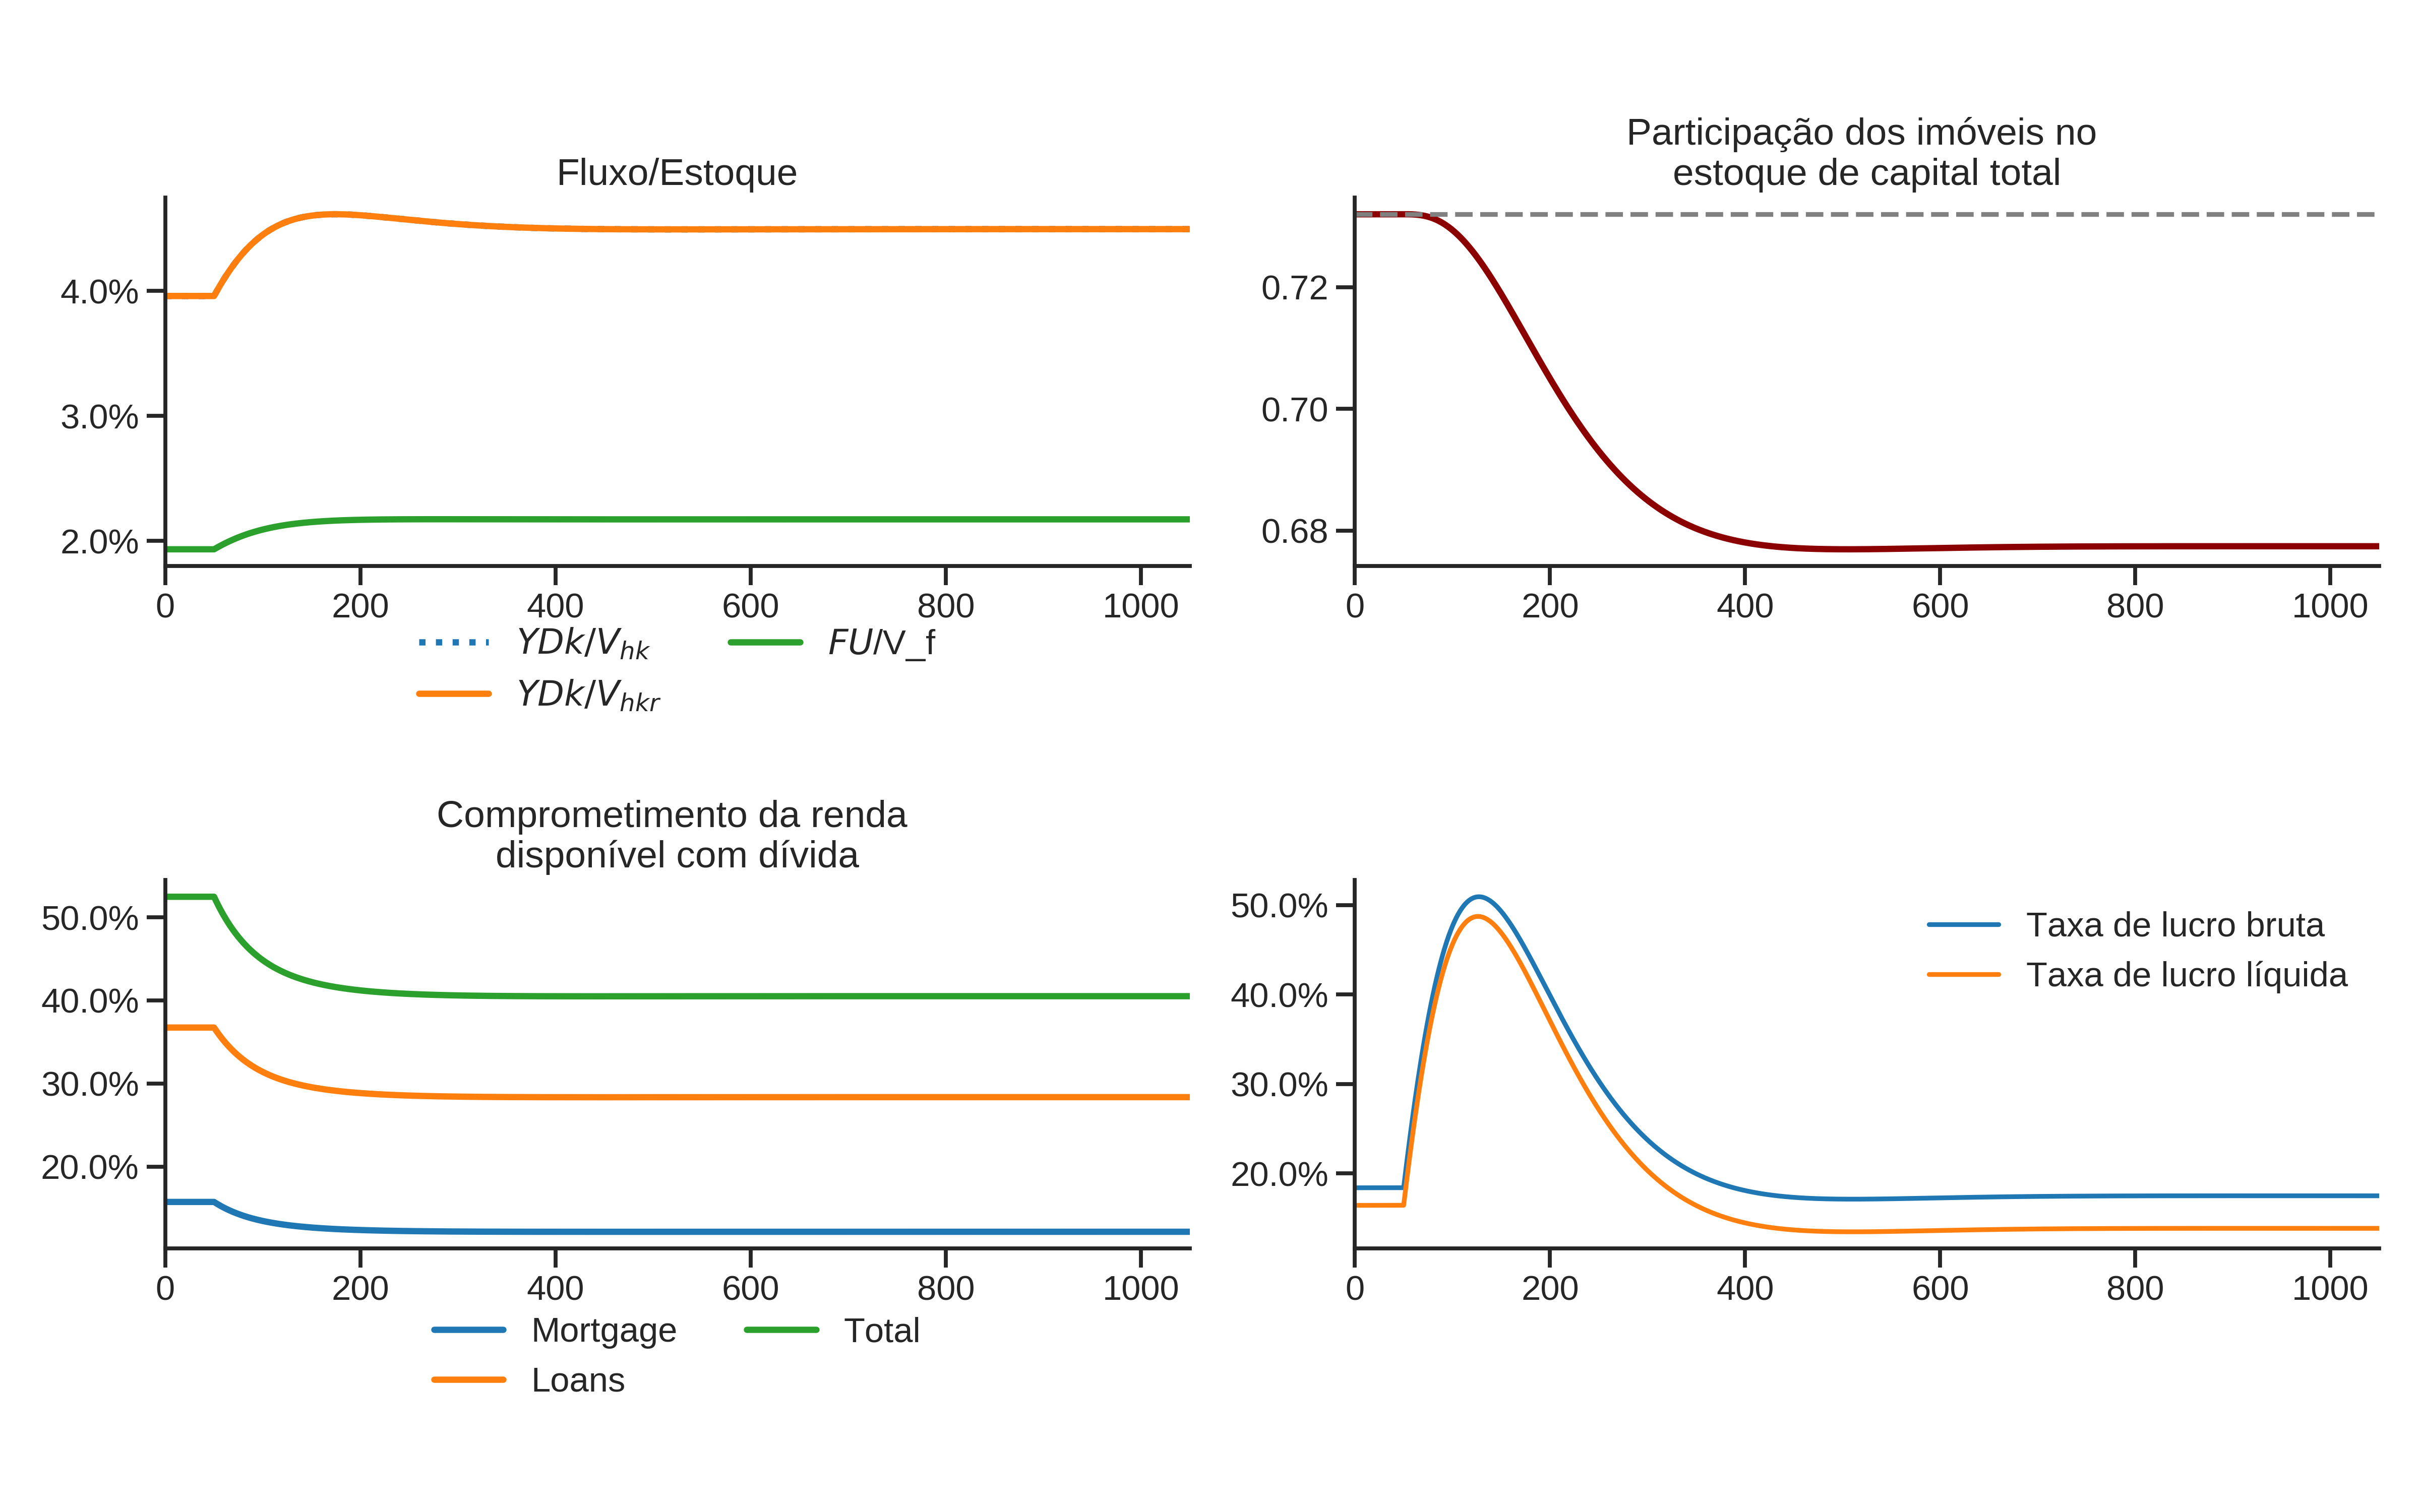
\includegraphics[width=\textwidth]{../../Modelo/Versoes/Shock_1Norms.png}
	\caption*{\textbf{Fonte:} Elaboração própria}
\end{figure}



Em resumo, tais resultados estão de acordo com \textcite{freitas_growth_2015} e explicitados nas figuras \ref{choque_1} e \ref{choque_4}. A especificidade do presente modelo, como destacado, é a existência de dois tipos de estoques de capital uma vez que as famílias também investem. Um resultado que pode parecer contraintuitivo é que uma maior taxa de crescimento do investimento residencial tem como resultado uma redução  da sua participação \textit{real} no estoque de capital total (isto é, diminuição de $k$) e tais resultados são iguais independentemente se a taxa de crescimento dos gastos autônomos aumenta por conta da inflação imobiliária ou de seu componente autônomo ($\phi_0$). 
A principal diferença na presença da inflação de imóveis é o crescimento da riqueza nominal das famílias mais acelerado que a renda disponível de modo que esta razão tende a zero no longo prazo tamanho aumento dos imóveis no portfólio dos capitalistas (figura \ref{choque_4Norms}).
%Adicionalmente, verifica-se um aumento  na participação nominal dos imóveis na presenção de inflação.


\begin{figure}[H]
	\centering
	\caption{Efeito de um aumento da inflação de imóveis}
	\label{choque_4Norms}
	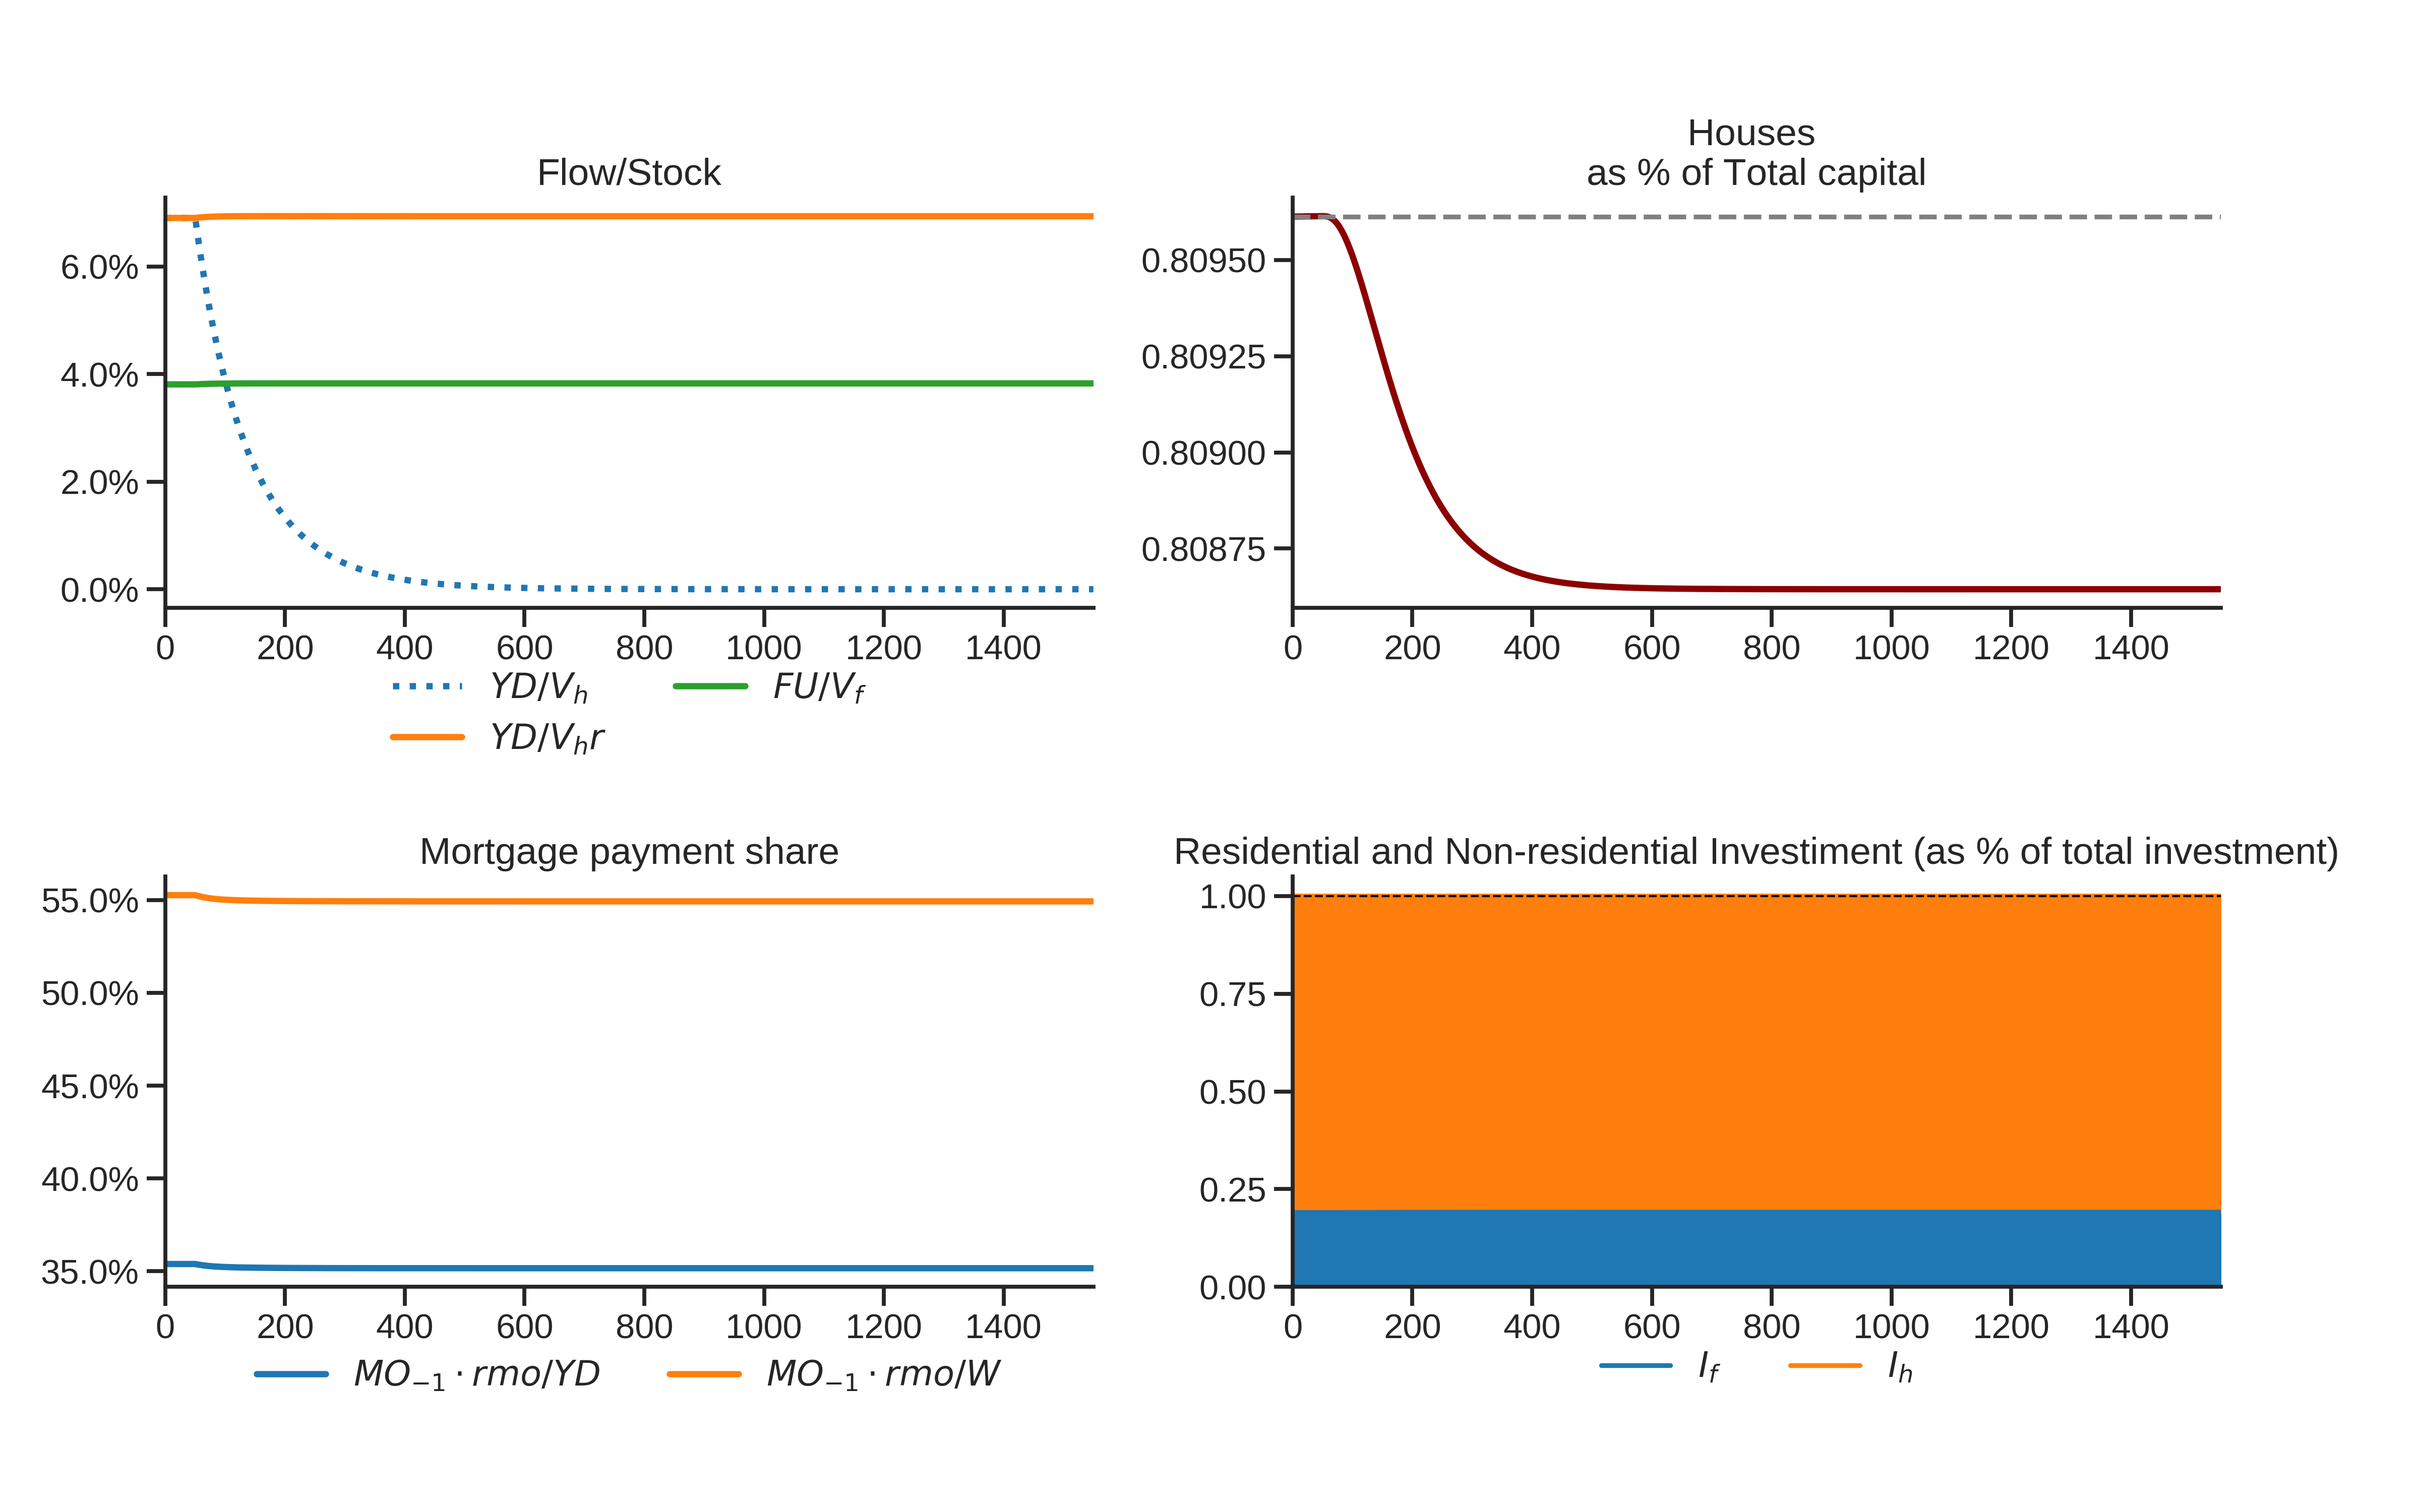
\includegraphics[width=\textwidth]{../../Modelo/Versoes/Shock_4Norms.png}
	\caption*{\textbf{Fonte:} Elaboração própria}
\end{figure}


\subsection*{Redução da participação dos salários na renda}
%esse parágrafo ficou bem confuso
%O aumento no \textit{wage-share} gera efeitos positivos sobre a taxa de crescimento da economia e também sobre o grau de utilização, conforme mostra a figura 6(a). No entanto, tais efeitos são temporários uma vez que a taxa de crescimento dos gastos autônomos não é alterada. Isso é refletido no aumento do grau de utilização mesmo estando abaixo do desejado em alguns períodos dada a convergência da taxa de crescimento da economia a $g_Z$ de modo que: (i) taxa de crescimento média é maior que a inicial, mas converge para $g_Z$ no longo prazo; (ii) o aumento na propensão marginal a investir é temporário e retorna ao valor do \textit{baseline}; (iii) grau de utilização converge ao normal mais rapidamente em relação ao choque anterior. 

A redução no \textit{wage-share} gera efeitos negativos sobre a taxa de crescimento da economia e também sobre o grau de utilização, conforme mostra a figura \ref{choque_2}. No entanto, tais efeitos são temporários uma vez que a taxa de crescimento dos gastos autônomos não é alterada. 
Como resultado deste efeito nível, a taxa de crescimento do investimento das firmas diminui e o mesmo vale para a propensão marginal a investir.
No entanto, como as firmas seguem o princípio do ajuste do estoque de capital e dada a taxa de crescimento dos gastos autônomos, a taxa de crescimento do investimento das firmas aumenta para que o grau de utilização convirja ao normal.
%TODO Rever
Em paralelo, o menor \textit{wage-share} faz com que o multiplicador diminua de modo que a participação dos gastos autônomos da renda aumente.
Com isso temos que: (i) a redução na propensão marginal a investir é temporária e retorna ao valor do \textit{baseline}; (ii) grau de utilização converge ao normal mais rapidamente em relação ao choque anterior; (iii) diminuição do multiplicador e respectivo aumento da participação dos gastos autônomos na renda sobretudo por conta do efeito nível negativo sobre o produto.


\begin{figure}[H]
	\centering
	\caption{Efeito de uma redistribuição de renda a favor dos lucros}
	\label{choque_2}
	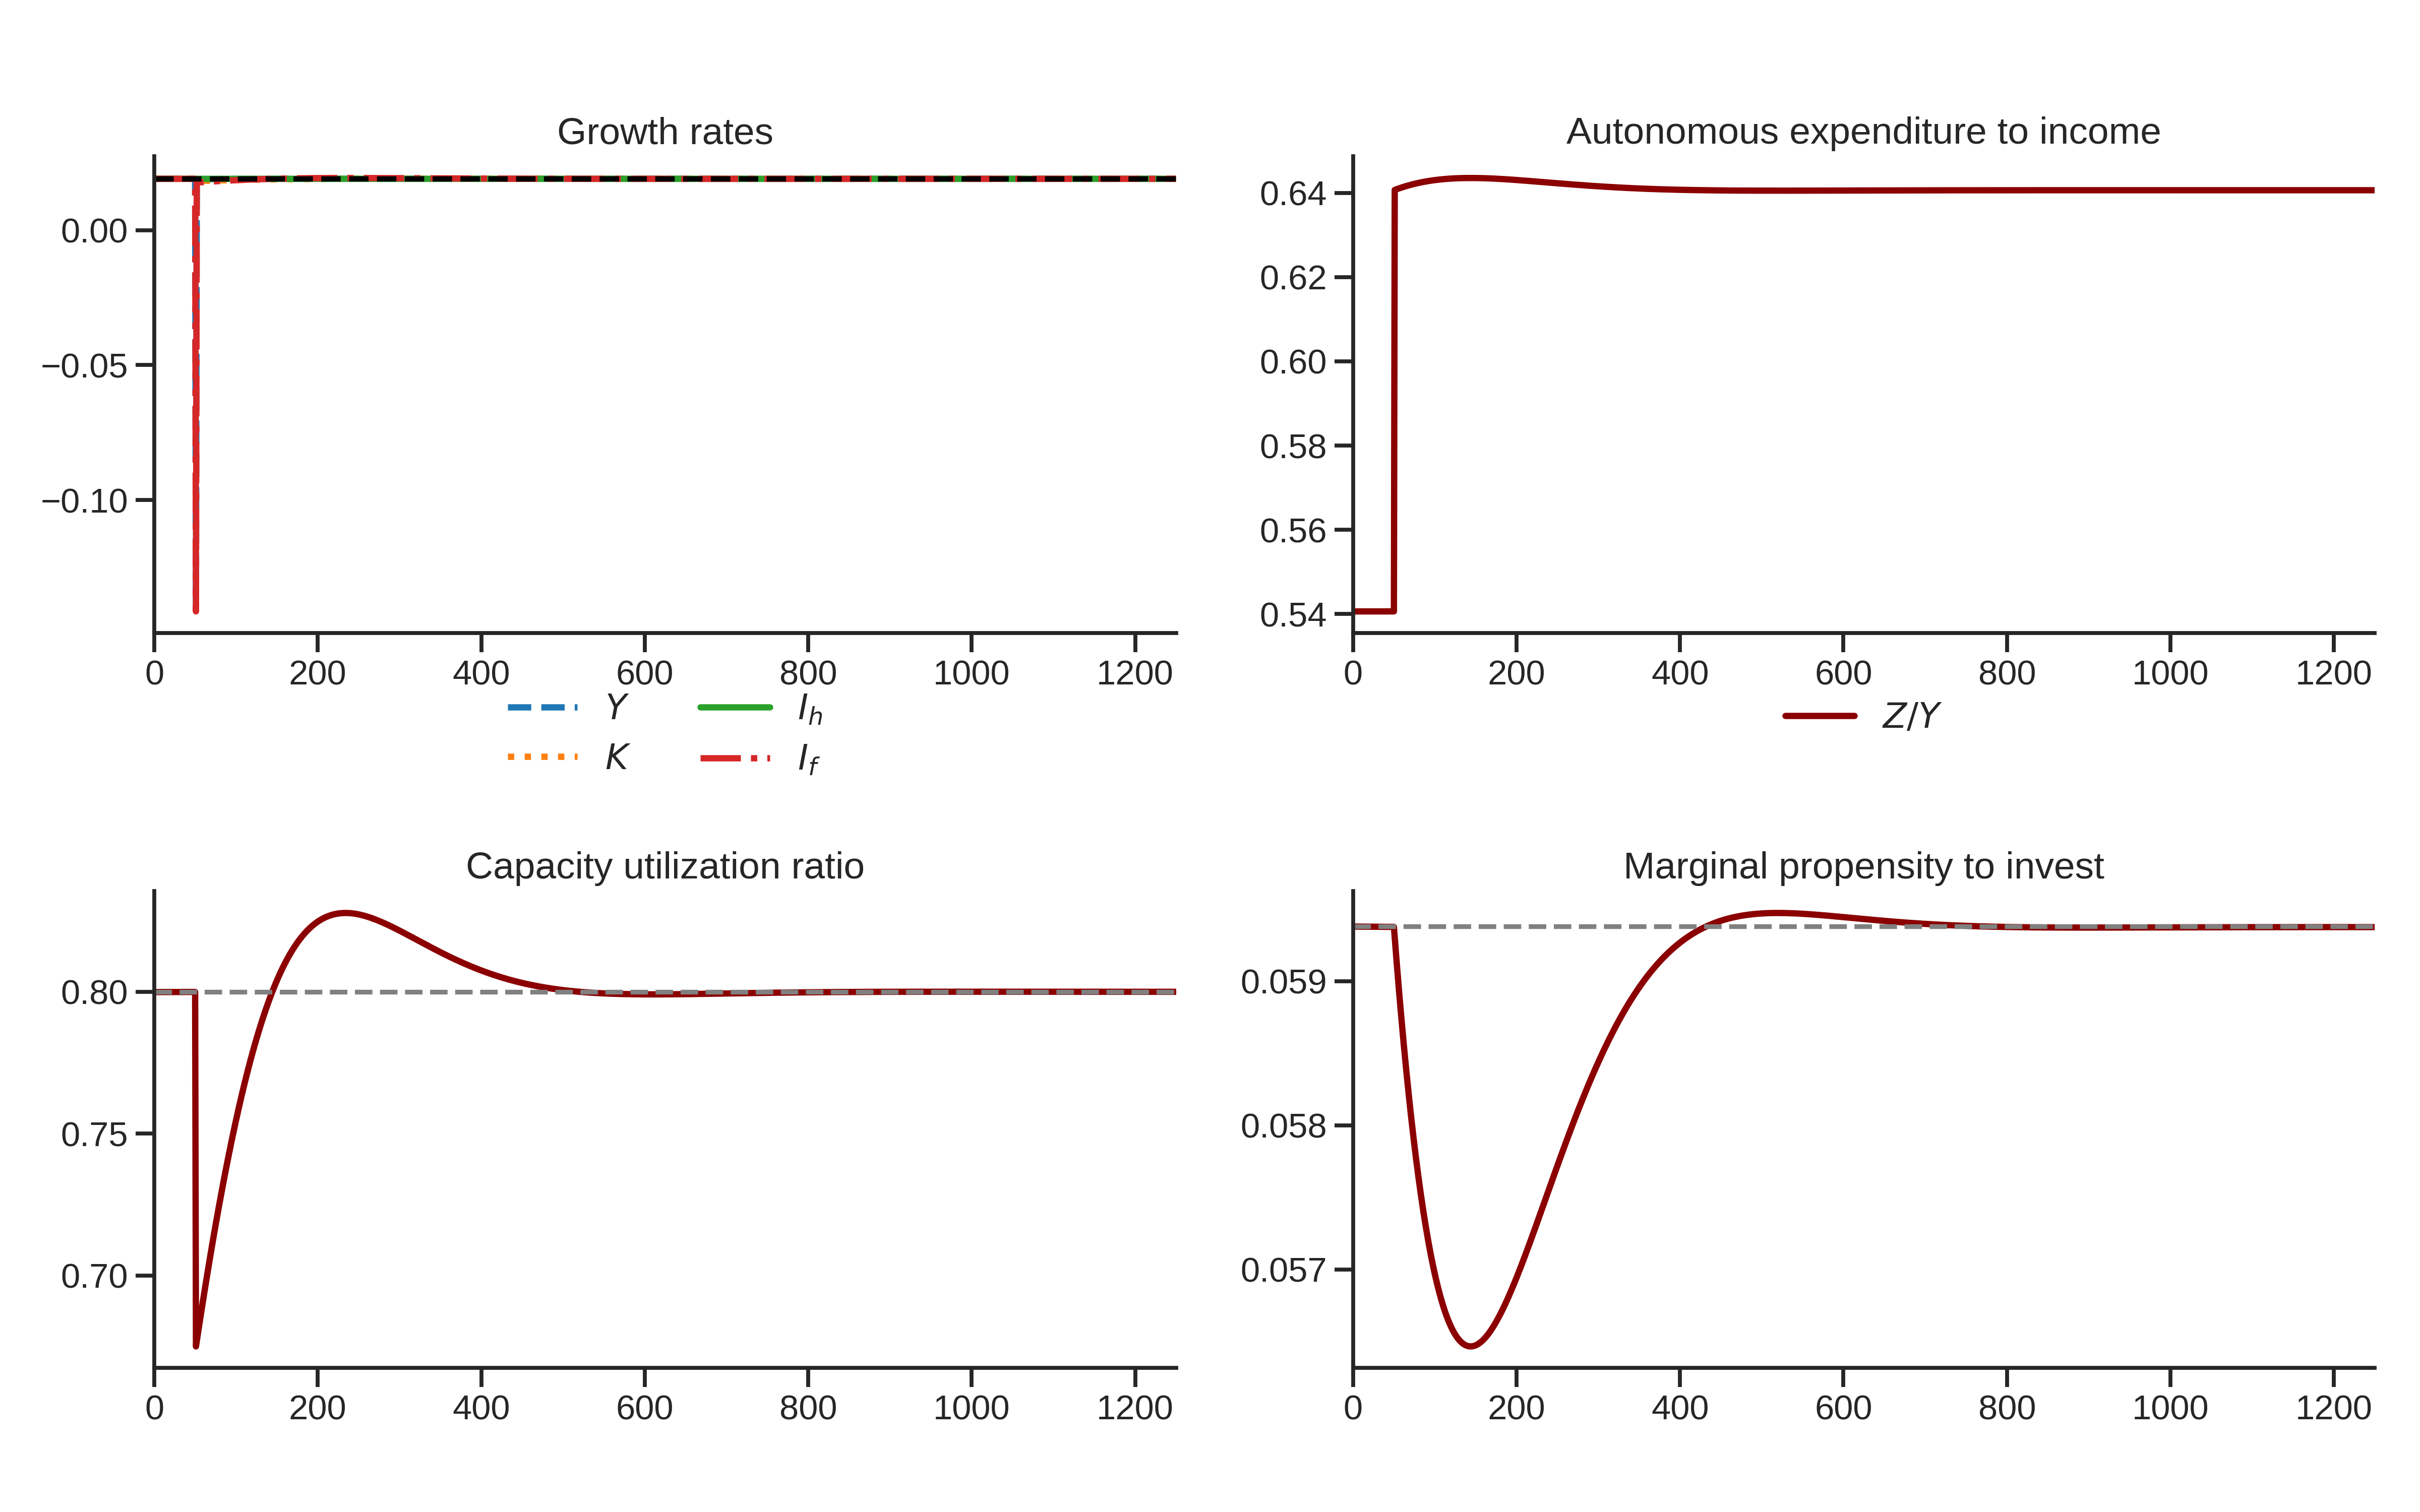
\includegraphics[width=\textwidth]{../../Modelo/Versoes/Shock_2.png}
	\caption*{\textbf{Fonte:} Elaboração própria}
\end{figure}

Por fim, apesar do efeito sobre a taxa de crescimento ser temporário, tem efeitos persistentes sobre a participação do capital das firmas no estoque total de capital da economia como indicado pela equação \ref{partial_omega}. Tal resultado decorre da menor taxa de acumulação no início do choque uma vez que a taxa de crescimento do investimento residencial é mantida constante. 
Outro efeito persistente é o maior comprometimento da renda das famílias com o pagamento de juros. 
Este resultado decorre da redução da massa de lucro dos capitalistas  --- apesar da maior participação dos lucros na renda --- associado ao efeito negativo no nível de renda e subsequente diminuição da renda diponível.
No entanto, como a taxa de crescimento do endividamento dos capitalistas não se altera --- dada a taxa de crescimento do consumo financiado por crédito ---, este aumento no \textit{profit-share} é seguido de um aumento na relação dívida/renda disponível das famílias capitalistas.
Em outras palavras, há um paradoxo na tentativa dos capitalistas aumentarem seu lucro --- por mudanças na margem de lucro e subsequente aumento no \textit{profits-hare} --- uma vez que gera um efeito negativo sobre o lucro líquido resultante do maior do comprometimento da renda disponível com o pagamento de juros dado o efeito nível negativo sobre a massa de lucro.
%TODO Grifar
Em relação às firmas, verifica-se uma aproximação permanente entre a taxa de lucro bruta e líquida das firmas resultante do efeito nível sobre o produto que fez com que a propensão marginal a investir diminuísse (temporariamente) de modo que a necessidade de financiamento deste setor também se reduzisse dada a política de distribuição de lucros (figura \ref{choque_2Norms}).

\begin{figure}[H]
	\centering
	\caption{Efeito de uma redistribuição de renda a favor dos lucros}
	\label{choque_2Norms}
	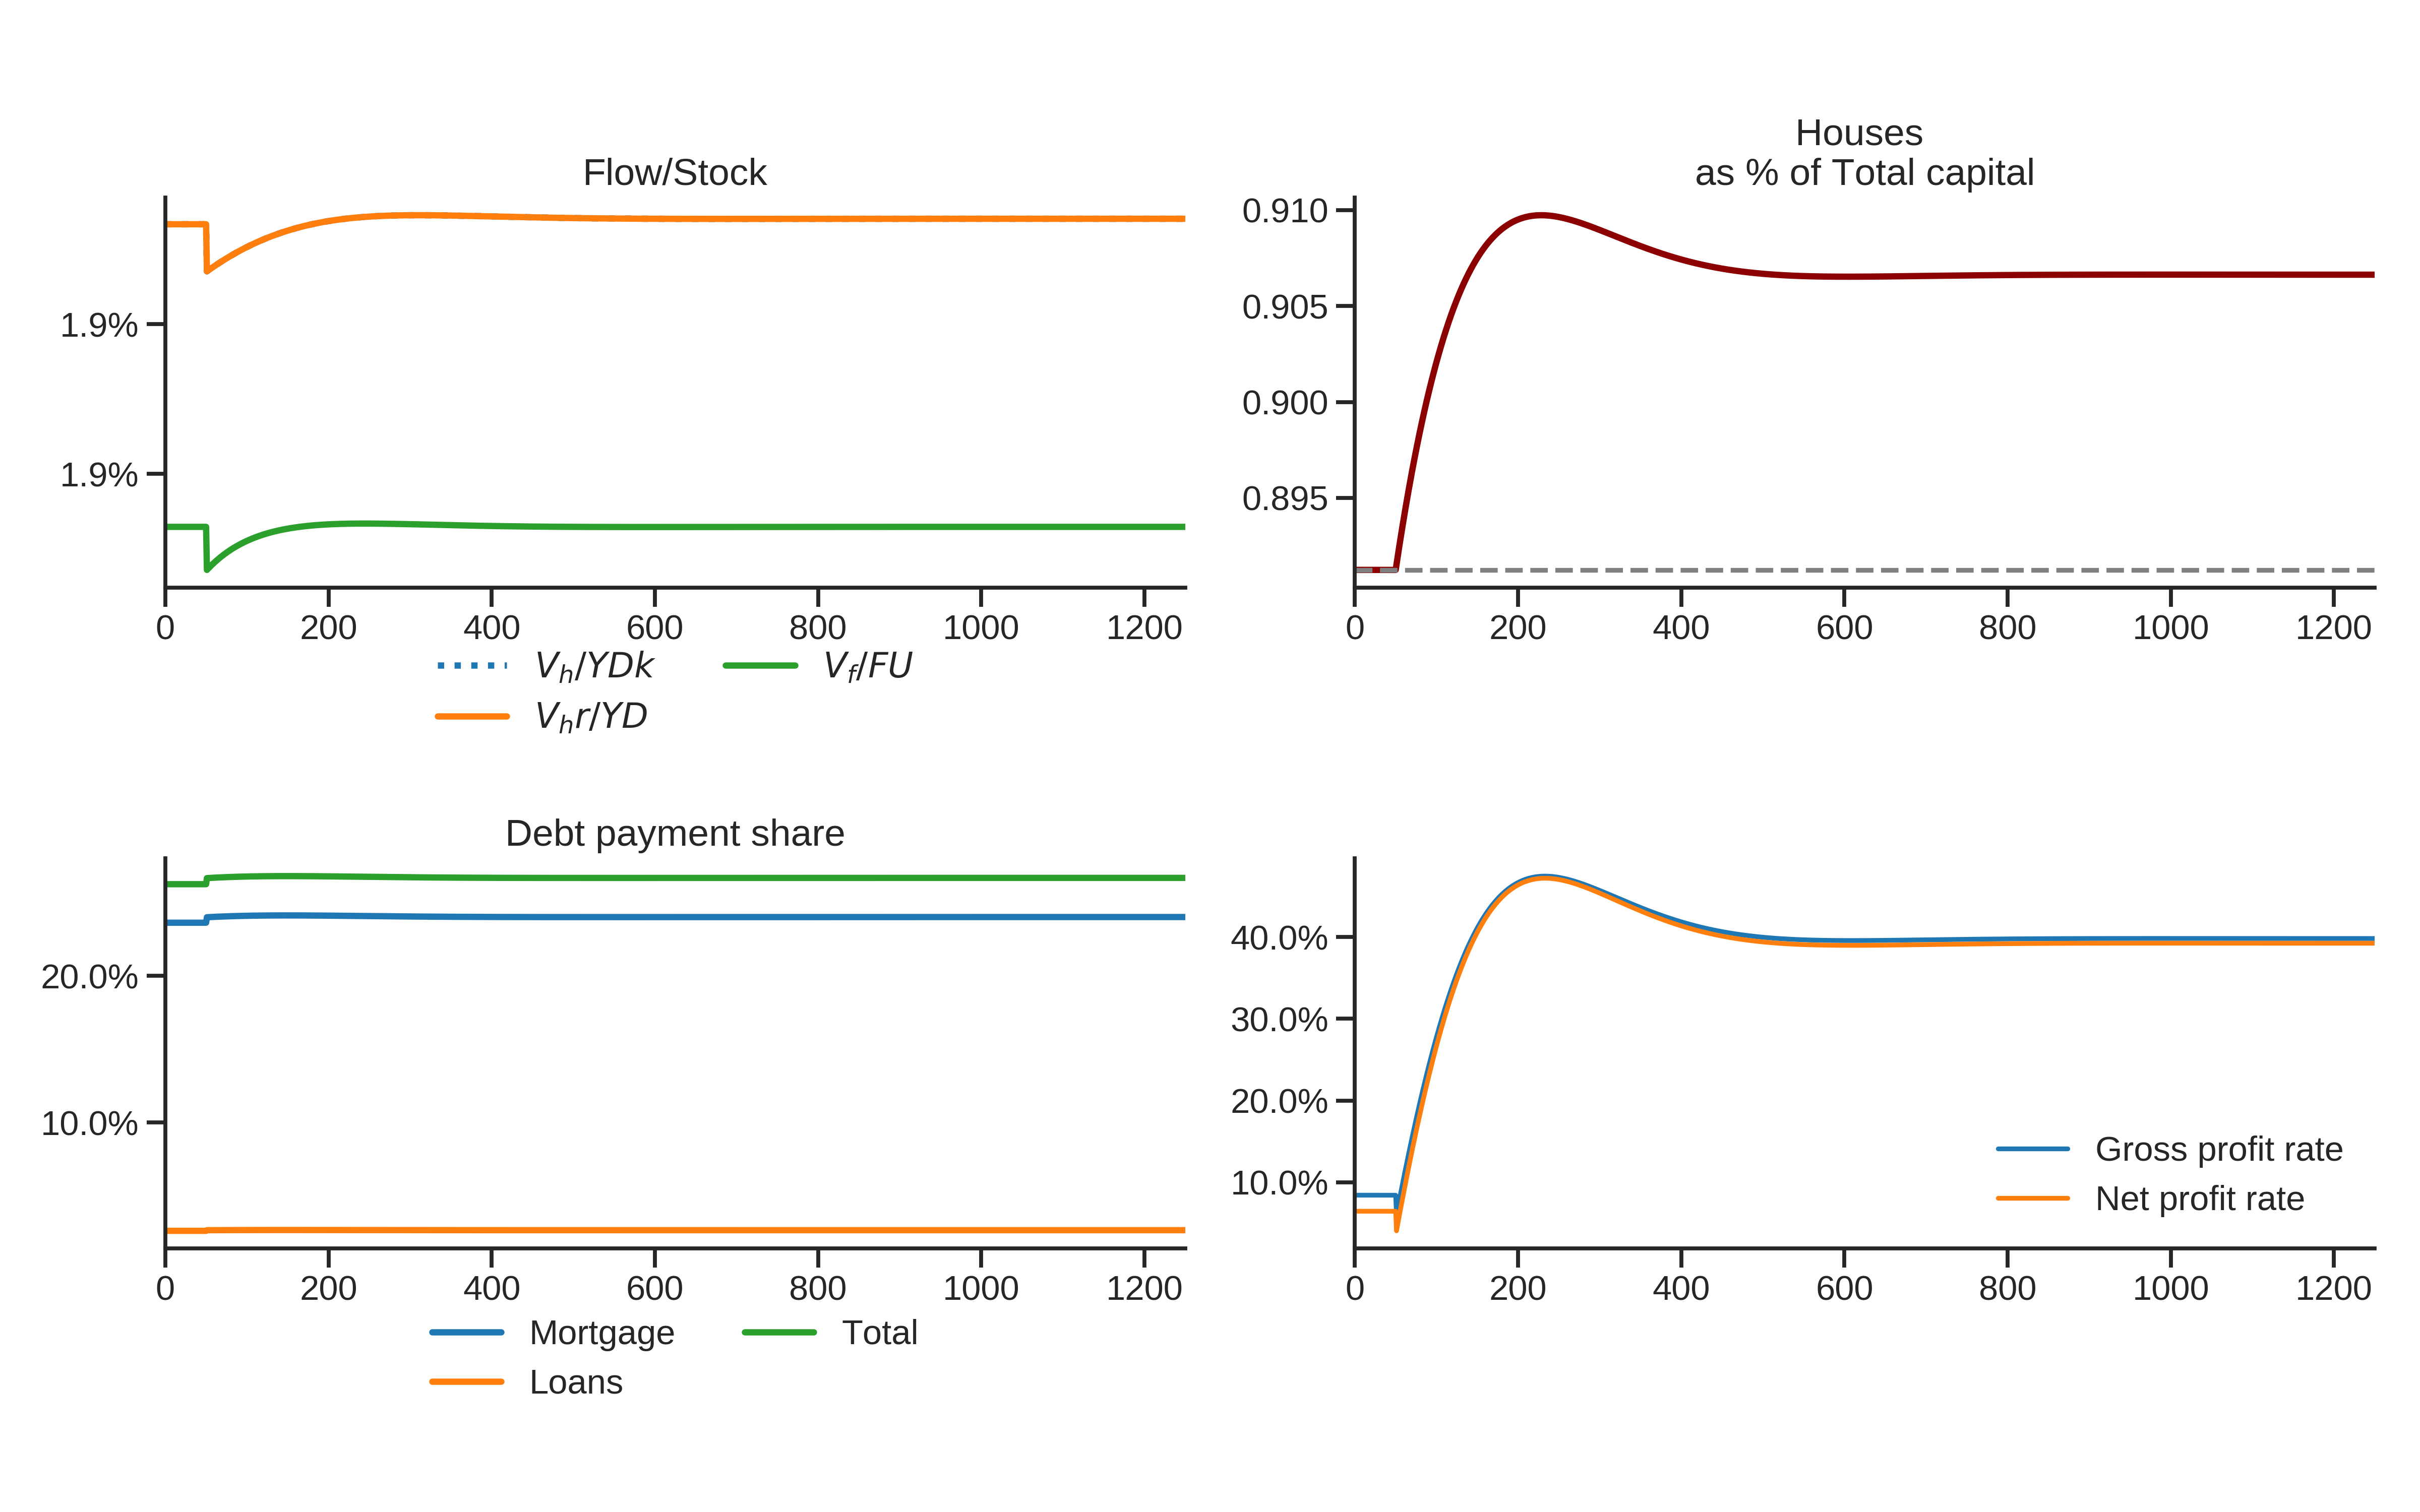
\includegraphics[width=\textwidth]{../../Modelo/Versoes/Shock_2Norms.png}
	\caption*{\textbf{Fonte:} Elaboração própria}
\end{figure}


\subsection*{Aumento da taxa de juros}

Um aumento na taxa de juros dos depósitos (e subsequente aumento das demais taxas de juros), ao impactar a taxa própria negativamente, possui efeitos persistentes sobre a taxa de crescimento (figura \ref{choque_3}). Como resultado da menor taxa de crescimento do investimento residencial, a taxa de crescimento do investimento das firmas diminui (\textit{overshooting} negativo) de tal modo que a participação dos imóveis no total do estoque de capital aumenta. 
Destaca-se ainda que os efeitos sobre as taxas de crescimento, a participação dos gastos autônomos, o grau de utilização e a propensão marginal a investir são simétricos em relação ao choque positivo na taxa de crescimento dos gastos autônomos e, por conta disso, dispensa uma análise mais pormenorizada (comparar o gráfico \ref{choque_3} com os gráficos \ref{choque_1} e \ref{choque_2}).
Dito isso, vale pontuar um resultado particular desta simulação referente ao comprometimento da renda das famílias capitalistas e do lucro das firmas com pagamento dos juros (figura \ref{choque_3Norms}). 
Tal resultado decorre da redução da taxa de crescimento da economia temporariamente superior a taxa de crescimento dos gastos autônomos.
Sendo assim, a diminuição da renda disponível dos capitalistas --- dada a queda da massa de lucro decorrente da redução do nível do produto --- é superior a redução do consumo financiado por crédito.
Essa relação causal seria, por si só, suficiente para que o comprometimento da renda disponível dos capitalistas com o pagamento de juros aumentasse, mas é acompanhada do aumento da própria taxa de juros, fazendo com que o efeito seja maior em relação à diminuição do \textit{wage-share}.
No que diz respeito às firmas, destaca-se não só a redução das taxas de lucro bruta e líquida como também um distanciamento entre ambas decorrente da maior necessidade de financiamento das firmas como consequência do aumento da taxa de juros e da diminuição da massa de lucro.
Por fim, conclui-se que a trajetória de endividamento das famílias capitalistas e das firmas é estável dado os valores dos parâmetros.

% hipotecários que não é acompanhado de um maior rendimento dos depósitos uma vez que está associado ao aumento do \textit{risk and trouble} e não da taxa básica de juros da economia.

\begin{figure}[H]
	\centering
	\caption{Efeito de Aumento na taxa de juros das hipotecas}
	\label{choque_3}
	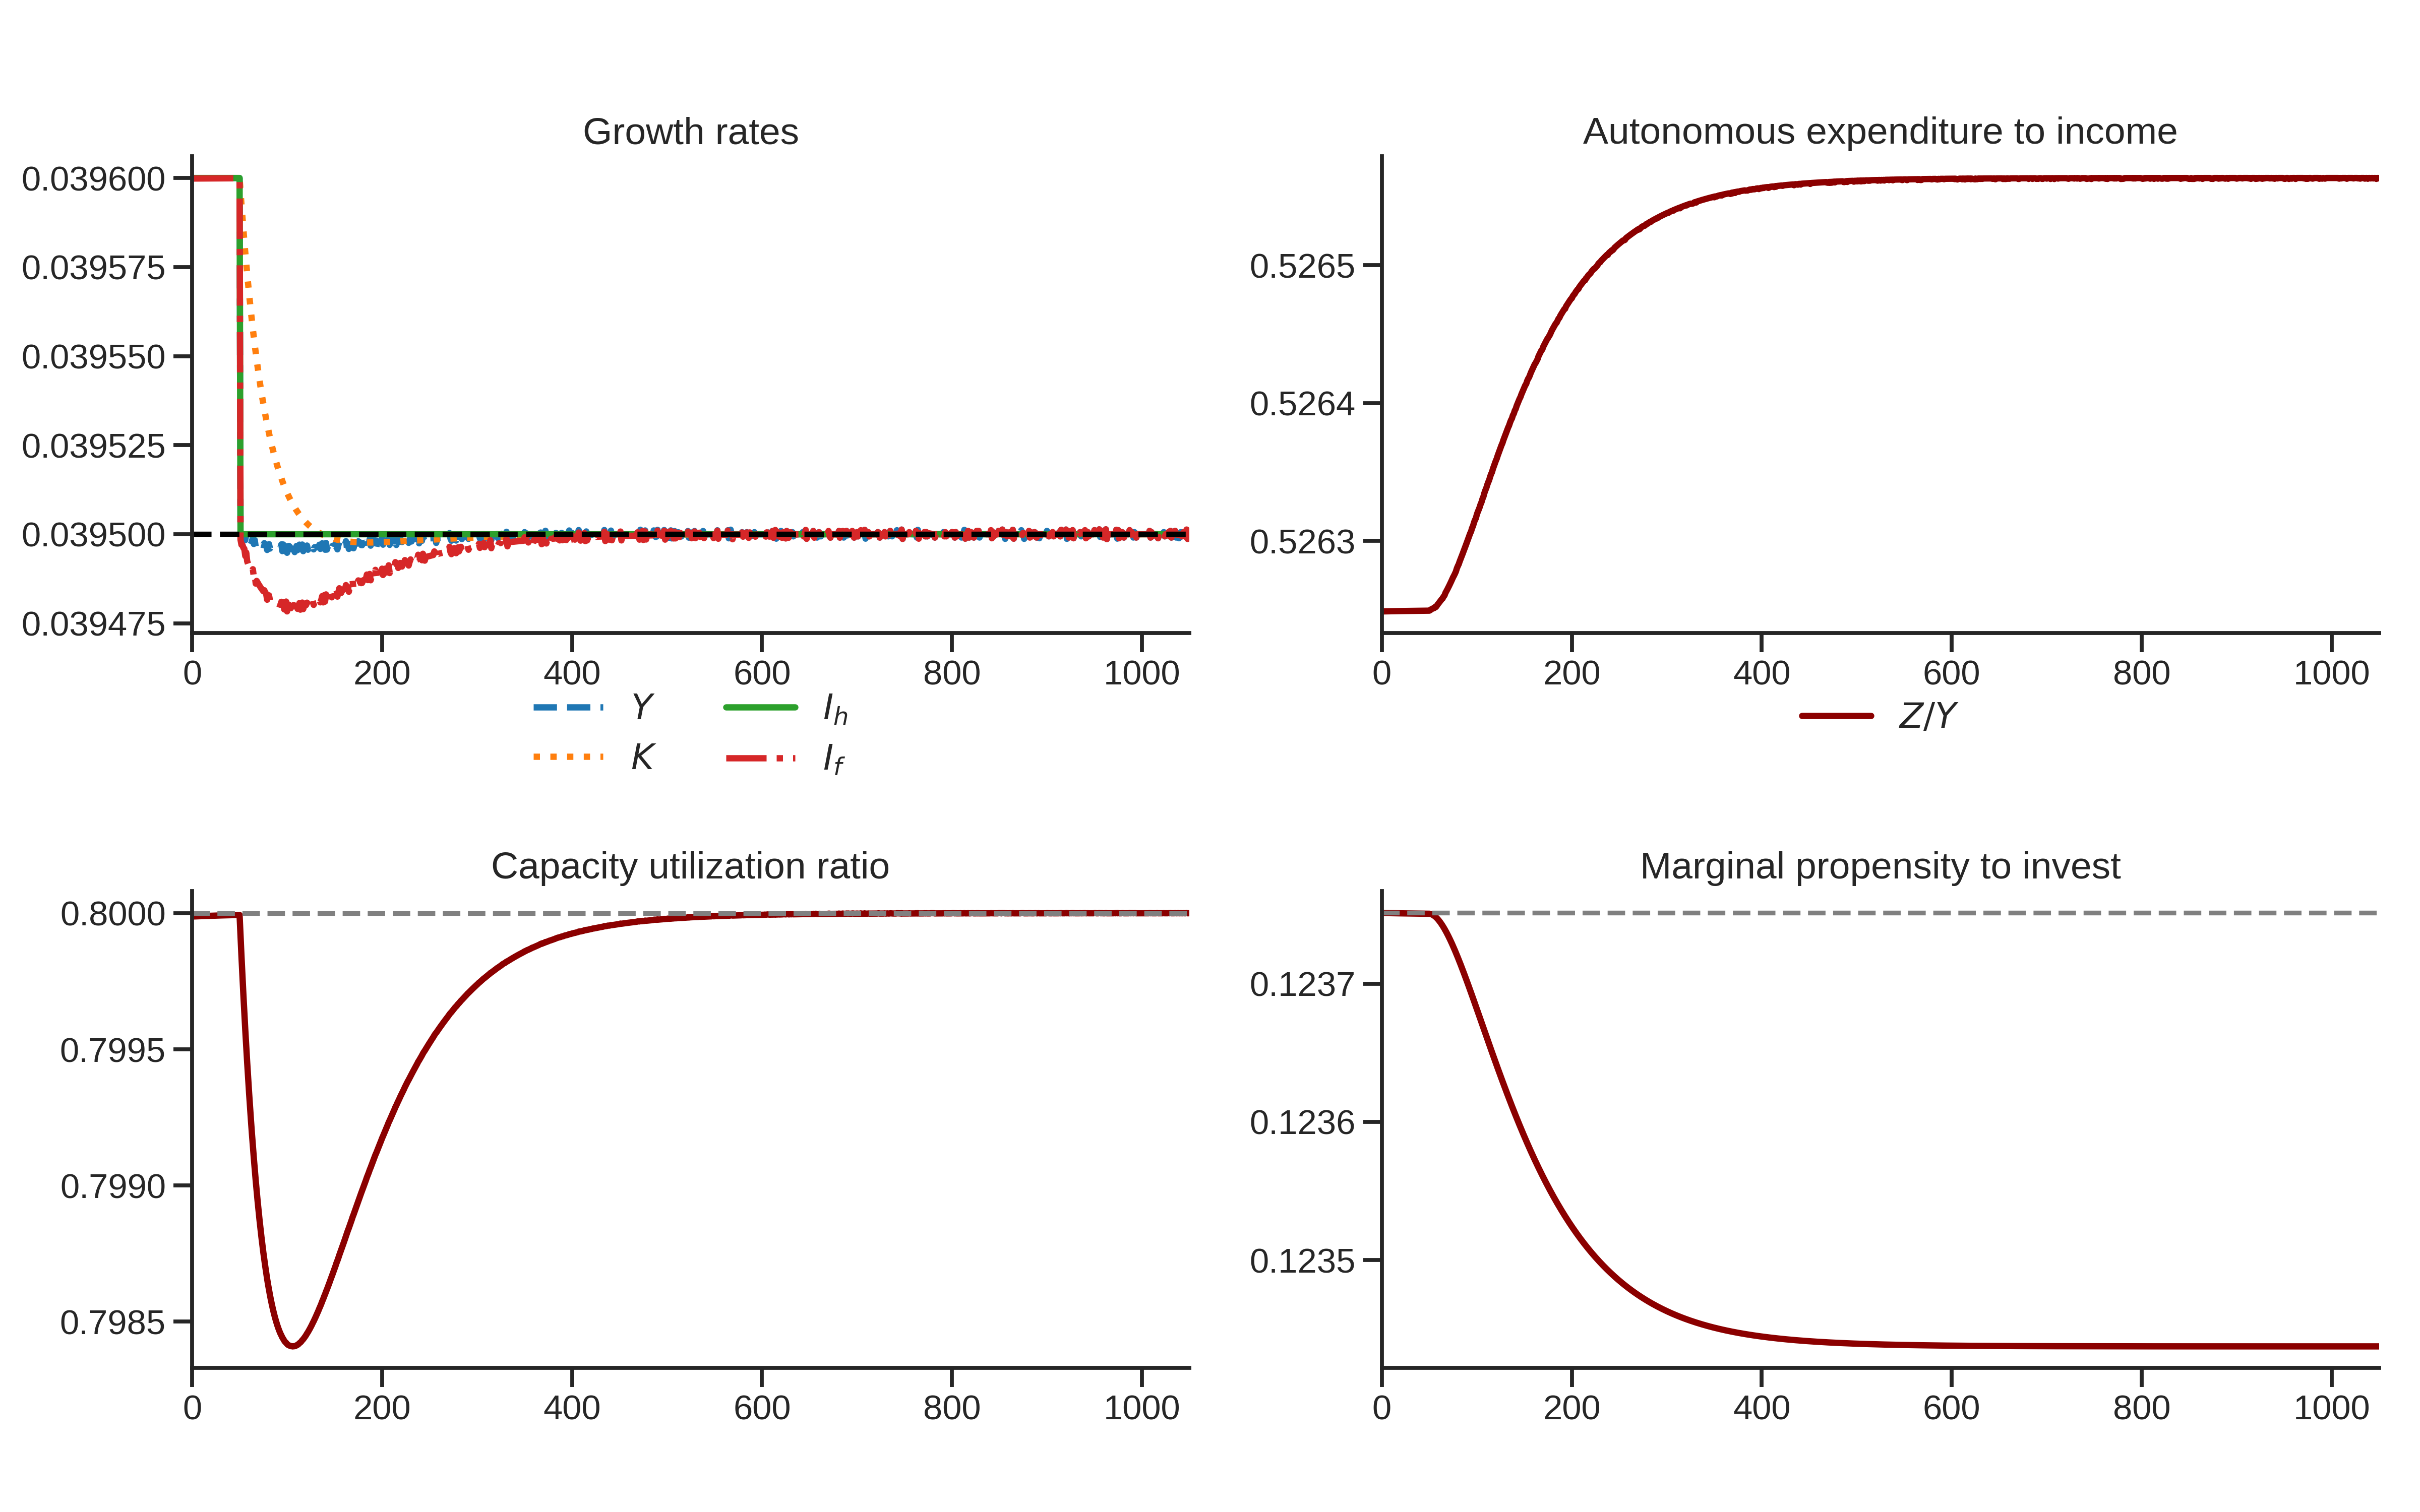
\includegraphics[width=\textwidth]{../../Modelo/Versoes/Shock_3.png}
	\caption*{\textbf{Fonte:} Elaboração própria}
\end{figure}


\begin{figure}[H]
	\centering
	\caption{Efeito de Aumento na taxa de juros das hipotecas}
	\label{choque_3Norms}
	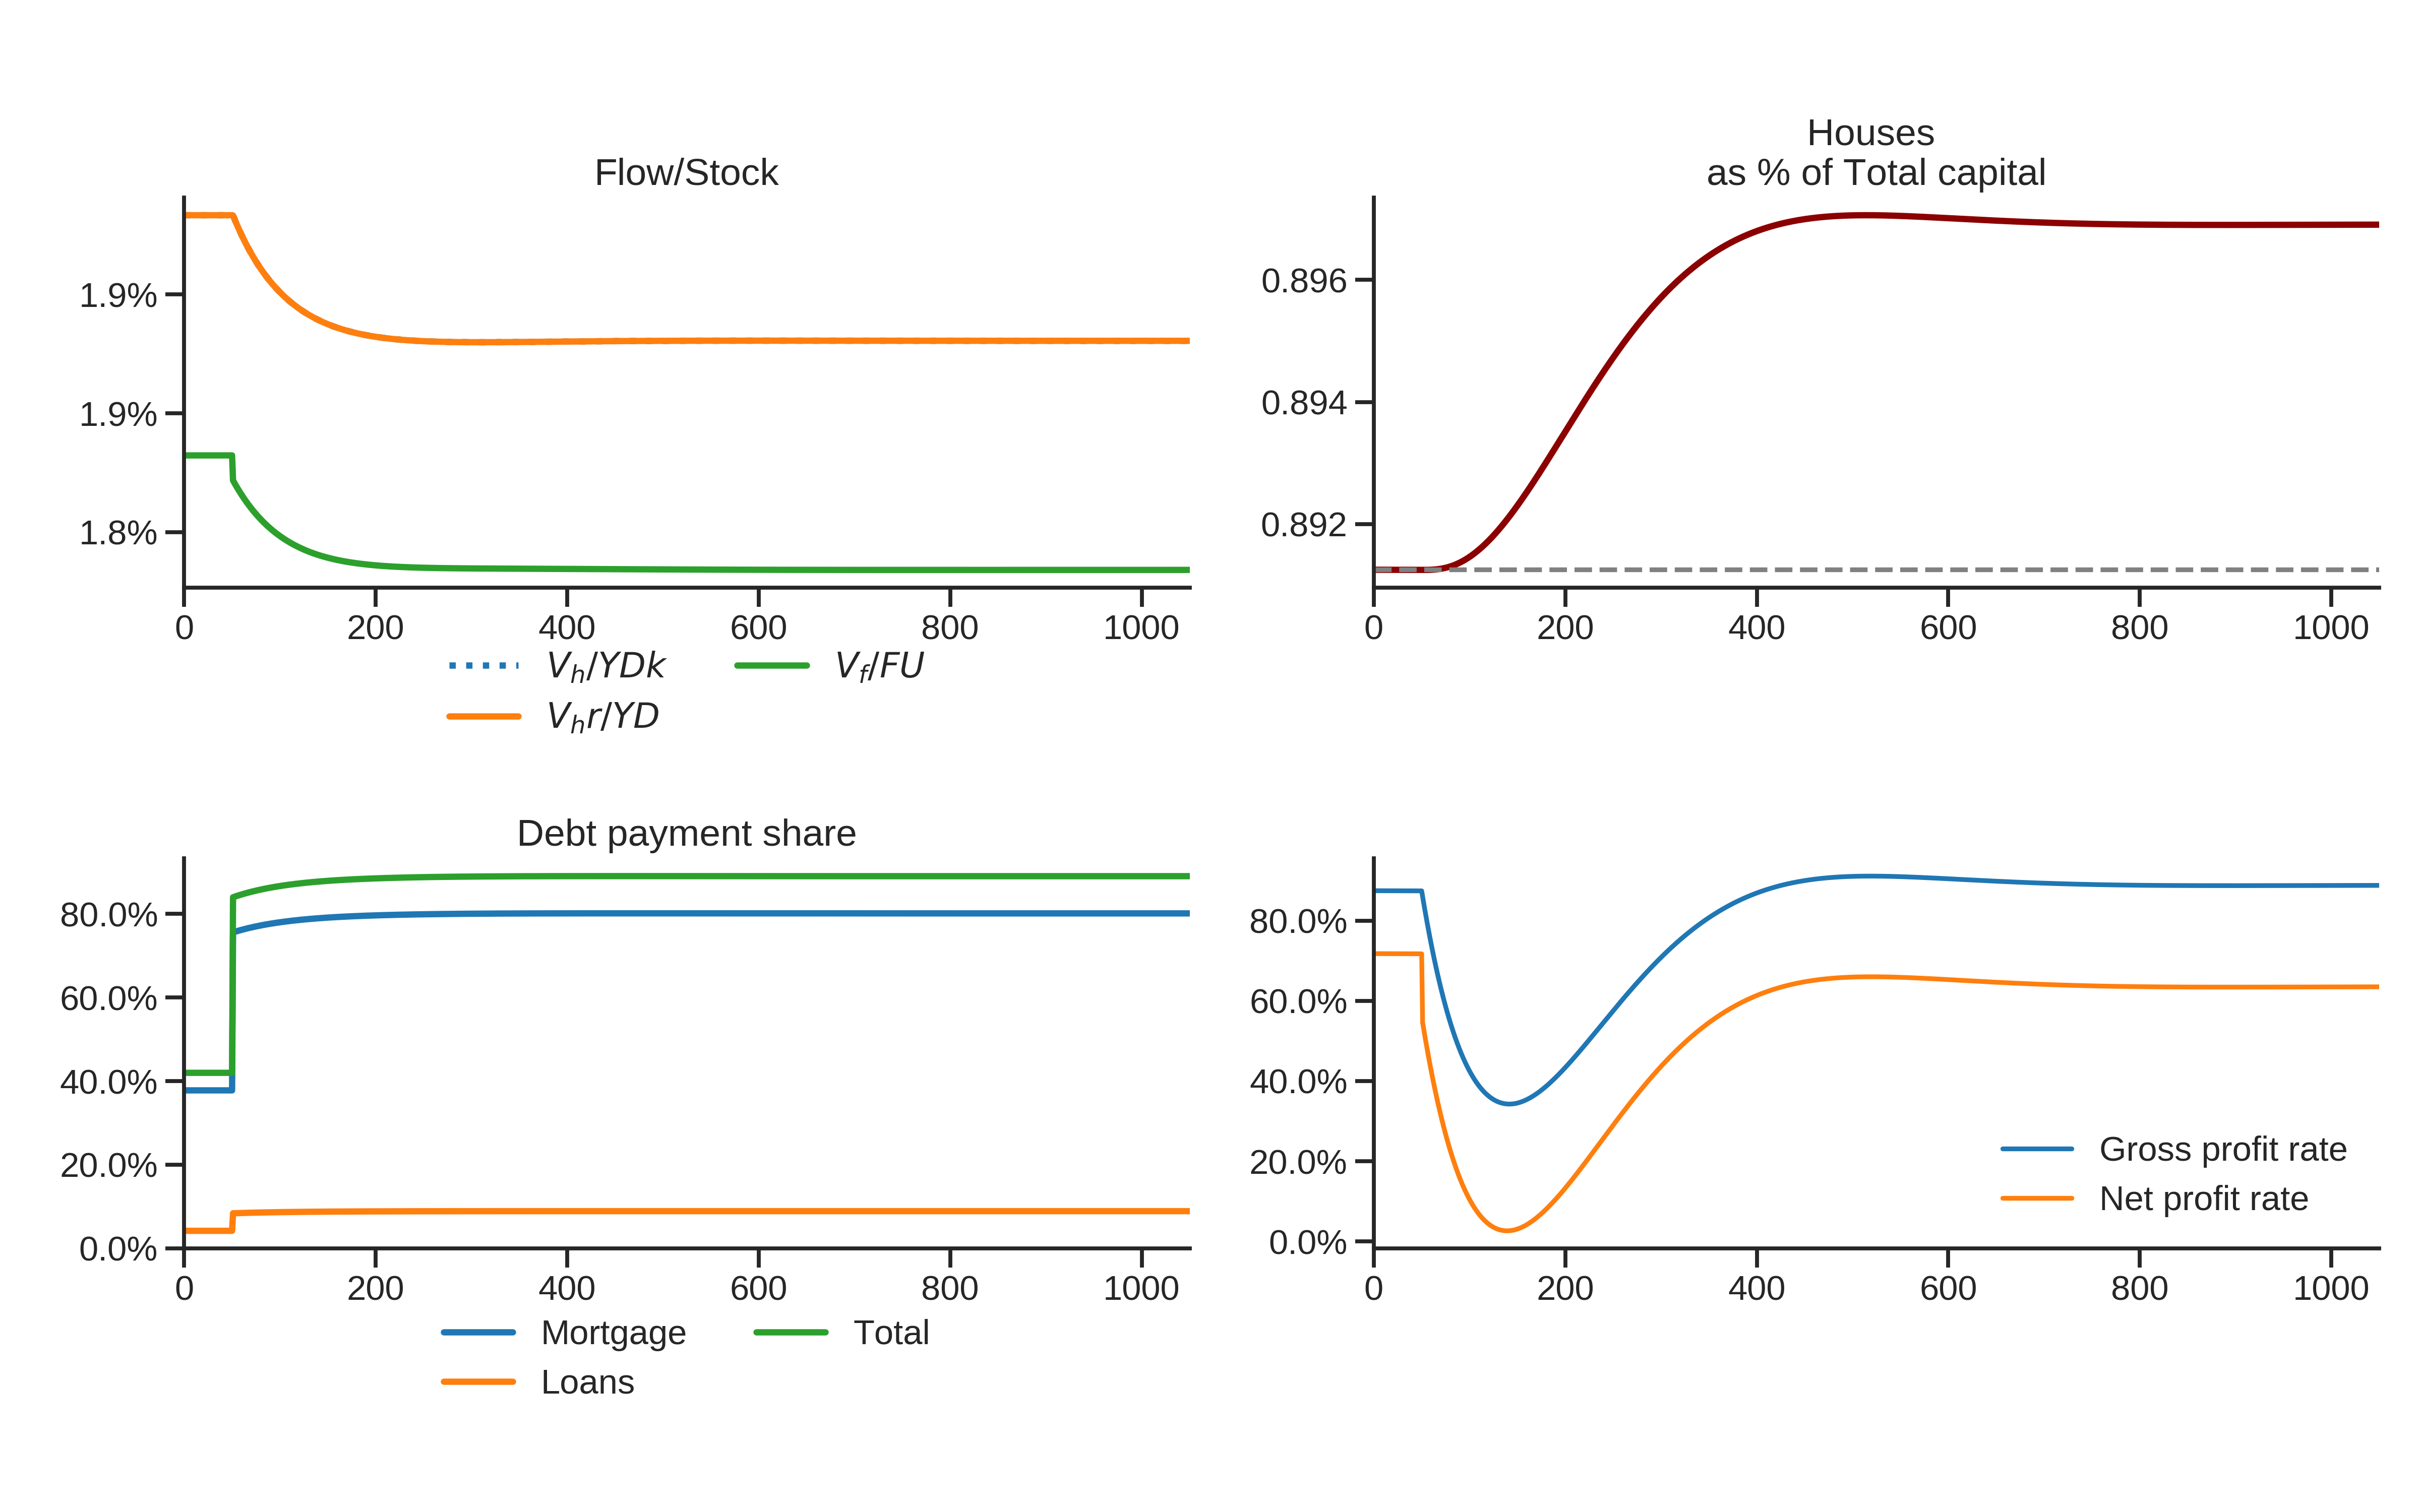
\includegraphics[width=\textwidth]{../../Modelo/Versoes/Shock_3Norms.png}
	\caption*{\textbf{Fonte:} Elaboração própria}
\end{figure}

% Please add the following required packages to your document preamble:
% \usepackage{multirow}
% \usepackage{graphicx}
\begin{table}[H]
	\centering
	\caption{Comparação dos choques ao \textit{baseline}}
	\label{ResumoChoques}
	%\resizebox{\textwidth}{!}{%
		\begin{tabular}{c|c|c|c|c||c|c|c|c}
			\hline\hline
			\multirow{2}{*}{} & \multicolumn{4}{c||}{\textbf{Médio prazo ($h \neq h^*$)}} & \multicolumn{4}{c}{\textbf{Longo prazo ($h = h^*$)}} \\ \cline{2-9} 
			& \textbf{$\Uparrow \phi_0$} & \textbf{$\Uparrow \pi$} & \textbf{$\Downarrow \omega$} & \textbf{$\Uparrow rm$} & \textbf{$\Uparrow \phi_0$} & \textbf{$\Uparrow \pi$} & \textbf{$\Downarrow \omega$} & \textbf{$\Uparrow rm$} \\ \hline
			\textbf{$g$} & + & + & - & - & + & + & 0 & - \\ \hline
			\textbf{$g_Z$} & + & + & 0 & - & + & + & 0 & - \\ \hline
			\textbf{$u$} & + & + & - & - & 0 & 0 & 0 & 0 \\ \hline
			\textbf{$h$} & + & + & - & - & + & + & 0 & - \\ \hline
			\textbf{$k$} & - & - & + & + & - & - & + & + \\ \hline
			\textbf{$\frac{Z}{Y}$} & - & - & + & + & - & - & + & + \\ \hline
			\textit{$\frac{(r_{mo}\cdot MO_{-1} + r_l\cdot L_{k_{-1}})}{YD_k}$} & - & - & + & + & - & - & + & + \\ \hline\hline
		\end{tabular}%
	%}
	\caption*{\textbf{Fonte:} Elaboração própria}
\end{table}


